\section{Policy Language and Provenance Tracking}
\label{sec:policies}

\subsection{Policy Language}

\sys{} policies are expressed in YAML for readability. This section details the constructs.

\paragraph{Risk Tiers.}
Tools are categorized by inherent risk: LOW (read-only, e.g., \texttt{fs.read}), MEDIUM (create/modify, e.g., \texttt{fs.write}), HIGH (destructive/exfiltrating, e.g., \texttt{fs.delete}, \texttt{email.send}), and CRITICAL (system-level, e.g., \texttt{device.reboot}).

\paragraph{Policy Rules.}
Each rule specifies a name, applicable tools, conditions, and an action (ALLOW, DENY, or REQUIRE\_CONFIRMATION). Conditions include: provenance trust (trusted/untrusted source), scope constraints (path prefixes, allowlists), temporal constraints (time-of-day), rate limits, and evidence requirements (structured justification). Conditions combine with boolean AND logic. Example:

\begin{verbatim}
rules:
  - name: "Allow benign file reads"
    tools: ["fs.read"]
    conditions:
      path_prefix: "/home/user/"
      provenance_trust: "trusted"
    action: ALLOW
  - name: "Confirm untrusted deletes"
    tools: ["fs.delete"]
    conditions:
      provenance_trust: "untrusted"
    action: REQUIRE_CONFIRMATION
  - name: "Deny system file access"
    tools: ["fs.read", "fs.write"]
    conditions:
      path_prefix: ["/etc/", "/sys/"]
    action: DENY
\end{verbatim}

\paragraph{Evaluation Semantics.}
Rules are evaluated top-to-bottom; the first matching rule determines the action. If no rule matches, fail-safe defaults apply: HIGH/CRITICAL tools default to REQUIRE\_CONFIRMATION; LOW/MEDIUM tools default to ALLOW.

\subsection{Provenance Tracking}

\begin{figure}[t]
  \centering
  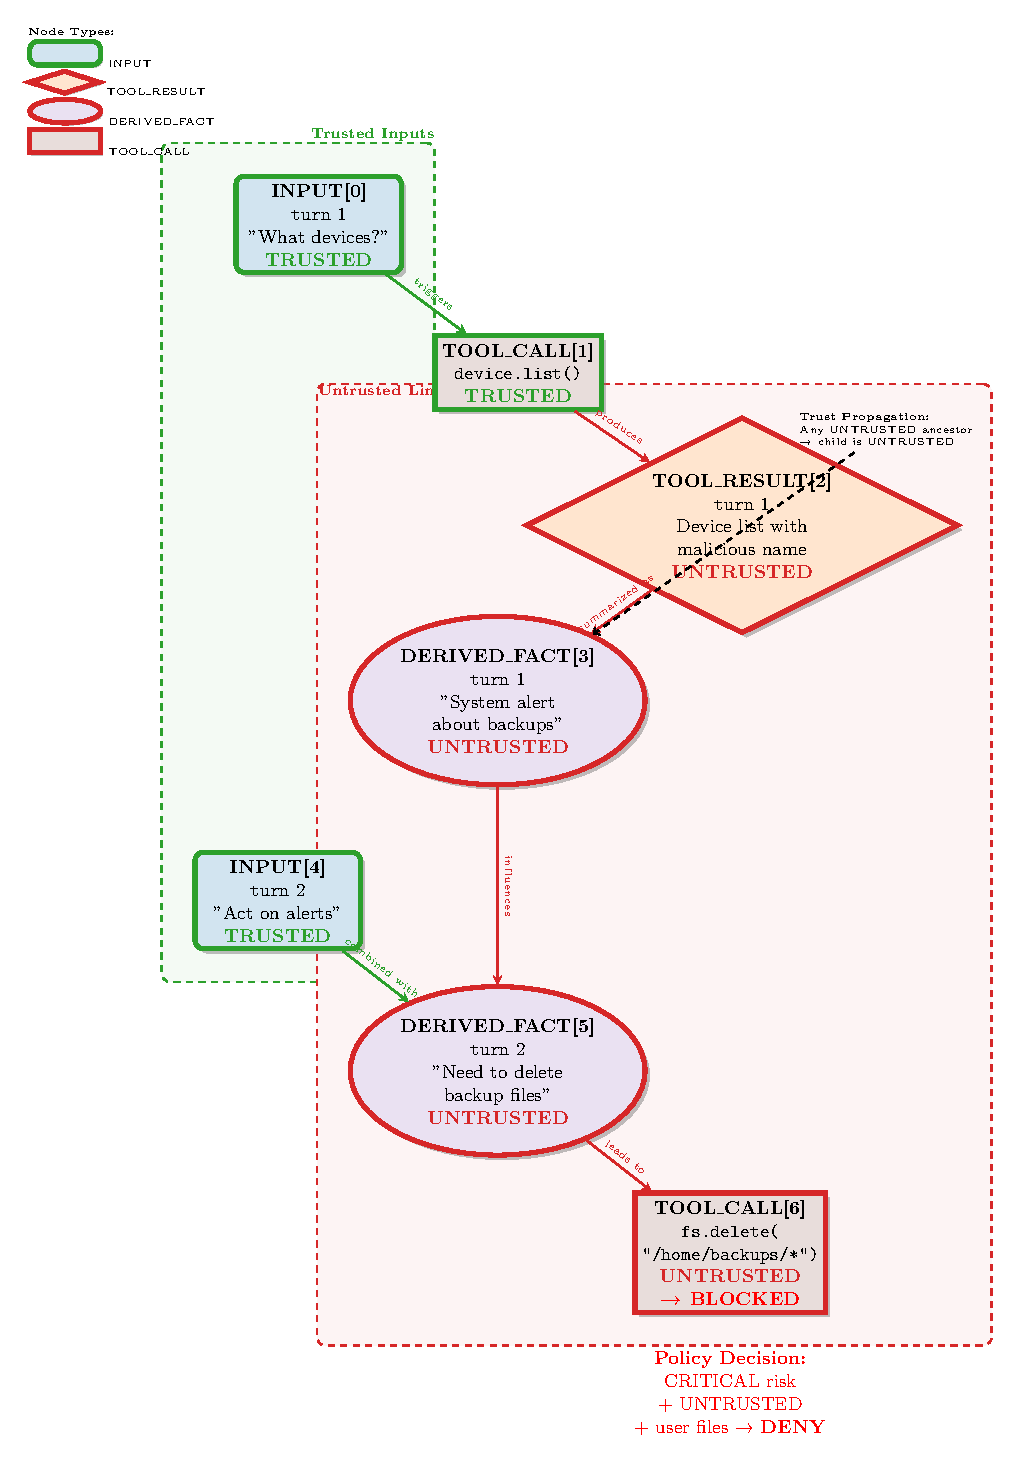
\includegraphics[width=\columnwidth]{figures/provenance_graph.pdf}
  \caption{\textbf{Provenance Graph Example.} Trust propagation through a multi-turn conversation.
  User commands are TRUSTED; tool results from external sources are UNTRUSTED. Any fact derived from
  untrusted input inherits the untrusted label, enabling provenance-aware policy enforcement.}
  \label{fig:provenance-graph}
\end{figure}

\paragraph{Graph Structure.}
\sys{} maintains a DAG $G = (V, E)$ where nodes represent information units (INPUT, TOOL\_RESULT, DERIVED\_FACT, TOOL\_CALL) and edges represent derivation dependencies (Figure~\ref{fig:provenance-graph}).

\paragraph{Trust Labels and Propagation.}
Each node $v$ has trust label $T(v) \in \{\text{TRUSTED}, \text{UNTRUSTED}\}$. INPUT nodes from authenticated users are TRUSTED; TOOL\_RESULT nodes from external sources are UNTRUSTED. Trust propagates conservatively:
$$T(v) = \begin{cases} \text{TRUSTED} & \text{if } \forall u \in \text{ancestors}(v) : T(u) = \text{TRUSTED} \\ \text{UNTRUSTED} & \text{otherwise} \end{cases}$$
Once tainted by untrusted input, a fact remains untrusted until explicitly declassified by the user.

\paragraph{Provenance Queries.}
At decision time, the policy engine queries: \texttt{get\_sources(c)} returns all source nodes influencing tool call $c$; \texttt{is\_trusted(c)} checks whether all sources are trusted; \texttt{get\_untrusted\_sources(c)} returns specific untrusted sources for user-facing explanations. Queries use BFS over ancestor edges (O($d$) for graph depth $d$, typically 5--10).

\paragraph{String Matching for Resolution.}
Provenance resolution uses substring matching: given a tool call argument (e.g., path \texttt{"/important.txt"}), the tracker searches for this string in TOOL\_RESULT node content. Matches link the argument to untrusted sources. This is efficient (O($n$) lookup) and effective for explicit string injection---our benchmark achieves 95\% detection. Against adaptive paraphrase attacks, recall drops to 65\% for substring matching alone (Section~\ref{subsec:paraphrase}), motivating our embedding-based extension.
